\documentclass{article}
\usepackage{graphicx} % Required for inserting images

\usepackage{float}
\usepackage{amsmath}
\title{Lesson 12 Homework - Proof Writing}
\author{William Wang}
\date{November 2025}

\begin{document}

\maketitle

\section{}
\subsection{}
\subsection{}
\subsection{}
\subsection{}
\begin{figure}[H]
    \centering
    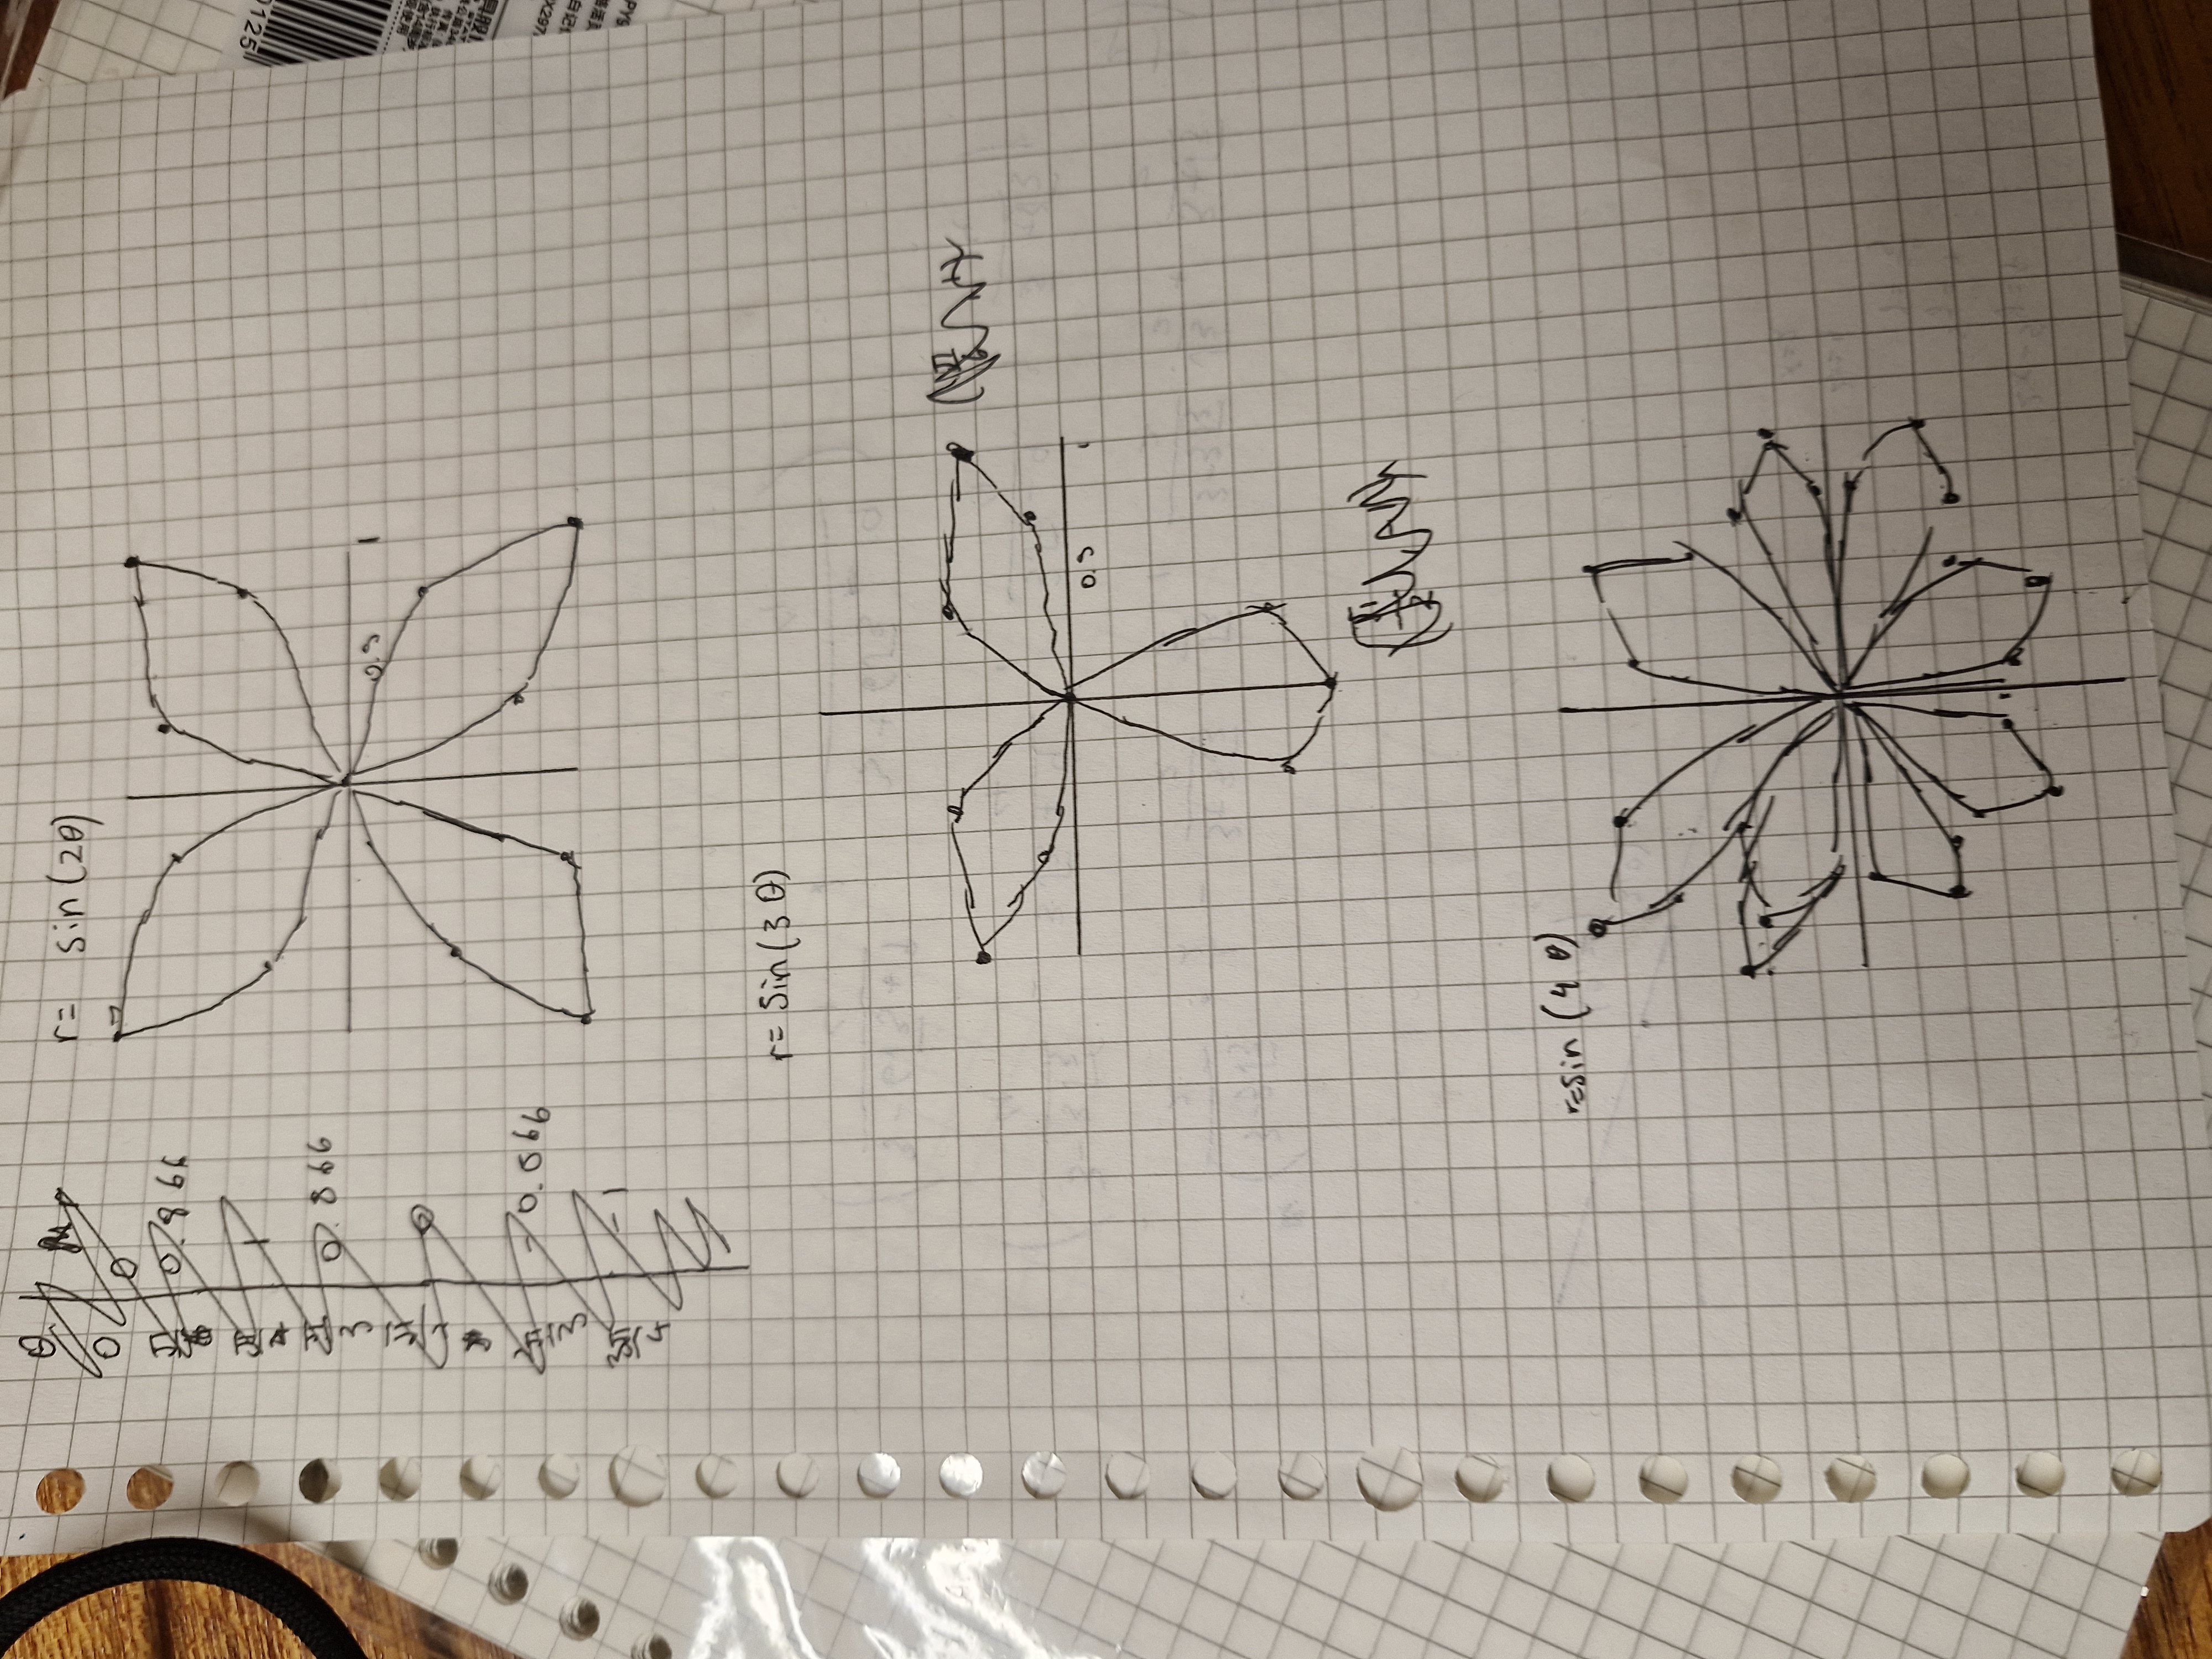
\includegraphics[width=0.75\linewidth]{1000006841.jpg}
\end{figure}
When there is 
\[r = \sin(k\theta)\]
If $k$ is odd, then there are k petals. If $k$ is even, then there are $2k$ petals
\section{}

\subsection{}
We want all possible values of $\theta$ such that $\overline{AO} \perp \overline{BO}$.

The direction of $\overline{AO}$ is $137^\circ + 180^\circ = 317^\circ$.

The direction of $\overline{BO}$ is $\theta + 180^\circ$.

Since the two segments are perpendicular,
\[
(\theta + 180^\circ) - (137^\circ + 180^\circ) \equiv \pm 90^\circ \pmod{360^\circ}.
\]
Simplifying,
\[
\theta - 137^\circ \equiv \pm 90^\circ \pmod{360^\circ}.
\]
Hence,
\[
\theta = 137^\circ \pm 90^\circ
\]
Therefore,
\[\theta = 47^\circ \text{ or } 227^\circ\]

\subsubsection{}
We now want all possible values of $\theta$ such that $\overline{AB} \perp \overline{AO}$.

The right angle is at $A$ in $\triangle OAB$.

Given:
\[
OA = 6, \quad OB = 12.
\]
By the Pythagorean theorem,
\[
OB^2 = OA^2 + AB^2 \implies AB^2 = 12^2 - 6^2 = 144 - 36 = 108,
\]
so
\[
AB = 6\sqrt{3}.
\]
Using the Law of Cosines at $O$:
\[
\cos(\angle AOB) = \frac{OA^2 + OB^2 - AB^2}{2(OA)(OB)} 
= \frac{36 + 144 - 108}{2(6)(12)} 
= \frac{72}{144} = \frac{1}{2}.
\]
Thus,
\[
\angle AOB = 60^\circ.
\]

Therefore, the difference in polar angles satisfies
\[
\theta - 137^\circ \equiv \pm 60^\circ \pmod{360^\circ}.
\]
Hence,
\[
\theta = 137^\circ \pm 60^\circ
\]
Therefore,
\[
\theta = 77^\circ \text{ or } 197^\circ
\]

\end{document}
